\chapter{无种子植物}\label{ch:g4:plants-without-seeds}

旧墙的背阴一面铺满了\omterm{prop:g4:plants-without-seeds:damp}{苔藓}；山毛榉树下，
\omterm{prop:g4:plants-without-seeds:damp}{蕨类}舒展开巨大的绿色羽叶。整个夏天去找找看：
你找不到花，找不到\omterm{prop:g3:flowers-fruits-seeds:transform}{果实}，也找不到\omterm{def:g2:from-seed-to-plant:seed}{种子}——
从来都找不到。然而\omterm{prop:g4:plants-without-seeds:damp}{苔藓}和\omterm{prop:g4:plants-without-seeds:damp}{蕨类}繁殖得相当好。
事实证明，\omterm{def:g1:plants-around-us:plant}{植物}产生下一代的方式
不止一种。

\section{蕨类和苔藓：孢子繁殖}

\begin{definition}[孢子]\label{def:g4:plants-without-seeds:spore}
\emph{孢子}\index{孢子}是一种微小的颗粒，数量极多，能从中长出新植株。
与\omterm{def:g2:from-seed-to-plant:seed}{种子}（\cref{def:g2:from-seed-to-plant:seed}）不同，
孢子只是一个单独的小点，\emph{内部没有养分储存，
也没有现成的小植株}——
它是最原始的生命起点。
\end{definition}

\begin{example}[蕨类羽叶之下]\label{ex:g4:plants-without-seeds:fern}
夏末翻开\omterm{prop:g4:plants-without-seeds:damp}{蕨类}的羽叶，背面排列着整齐的褐色小点。
每个小点都是一个\omterm{def:g4:plants-without-seeds:spore}{孢子}囊，里面装着成千上万个\omterm{def:g4:plants-without-seeds:spore}{孢子}；
\omterm{def:g4:plants-without-seeds:spore}{孢子}囊成熟后裂开，\omterm{def:g4:plants-without-seeds:spore}{孢子}随风飘散，像最细的尘埃。
落在潮湿阴暗地面上的\omterm{def:g4:plants-without-seeds:spore}{孢子}，
可以逐步长成一株新的\omterm{prop:g4:plants-without-seeds:damp}{蕨类}。
\end{example}

\begin{omfigure}
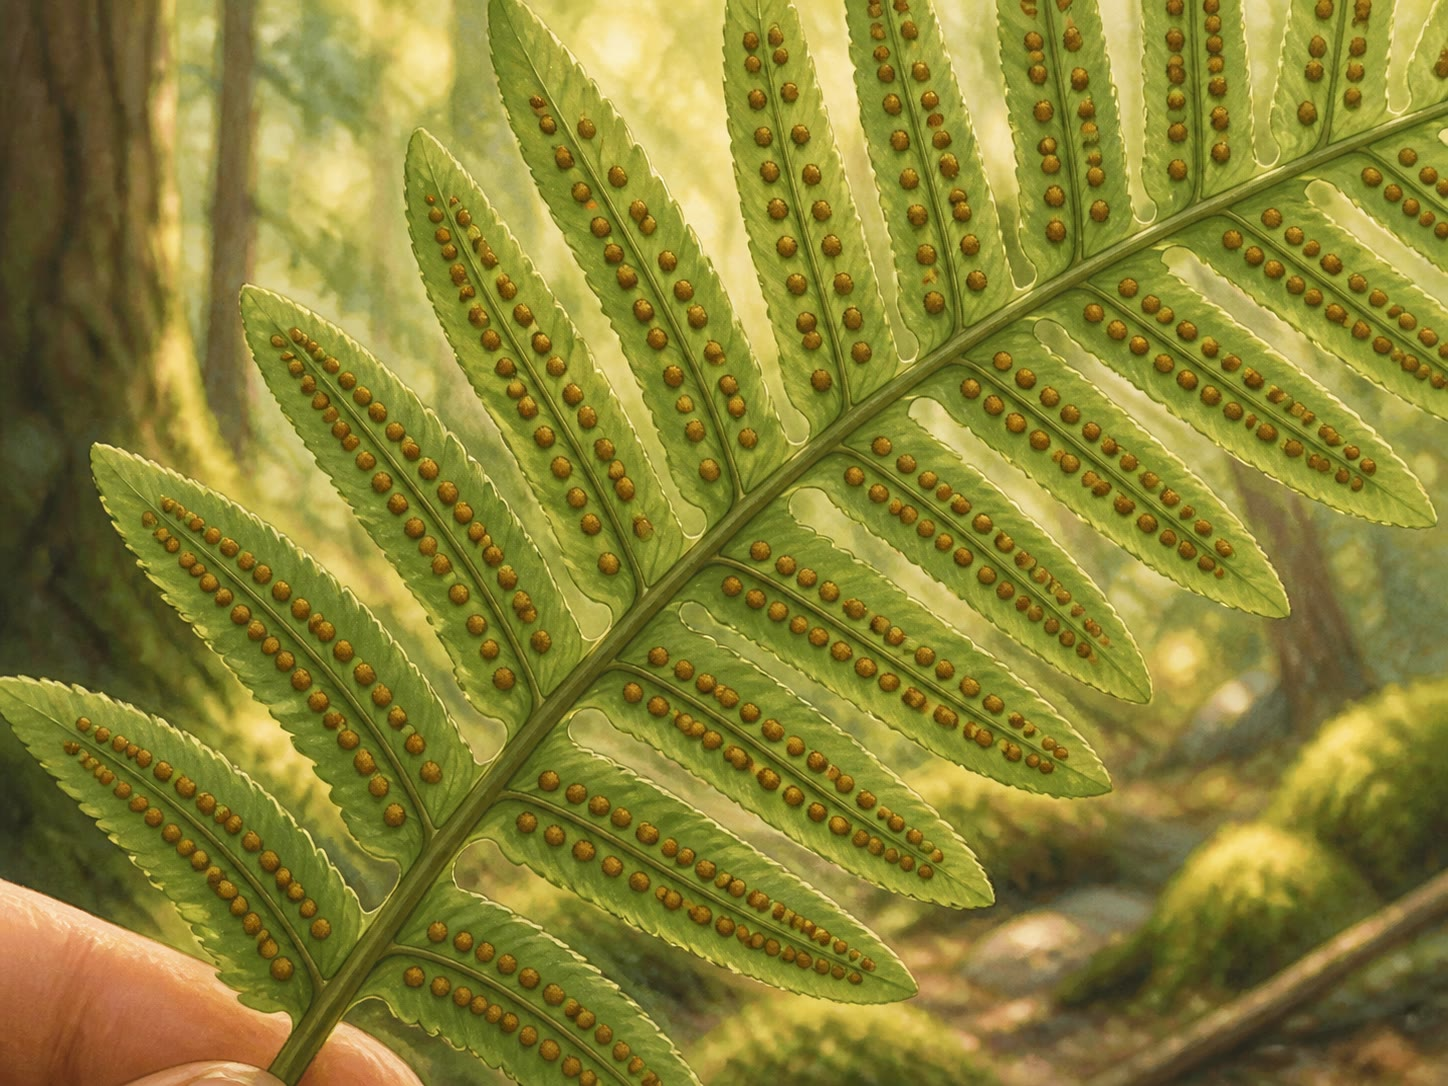
\includegraphics[width=0.56\linewidth]{images/book1/ai/g4-ferns-sori.jpg}

{\small 羽叶背面：整齐排列的褐色小点，
每一个都是装着成千上万个\omterm{def:g4:plants-without-seeds:spore}{孢子}的\omterm{def:g4:plants-without-seeds:spore}{孢子}囊。}
\end{omfigure}

\begin{proposition}[孢子植物需要潮湿]\label{prop:g4:plants-without-seeds:damp}
\omterm{def:g4:plants-without-seeds:spore}{孢子}\omterm{def:g1:plants-around-us:plant}{植物}——\emph{苔藓}\index{苔藓}和\emph{蕨类}\index{蕨类}——
只能在\emph{潮湿}的地方繁殖：它们的\omterm{def:g4:plants-without-seeds:spore}{孢子}，
以及由\omterm{def:g4:plants-without-seeds:spore}{孢子}长出的脆弱阶段，遇到干燥空气便会失水死亡。
这就是为什么\omterm{prop:g4:plants-without-seeds:damp}{苔藓}总是长在背阴的北墙上，
而从不长在向阳的南墙上，
\omterm{prop:g4:plants-without-seeds:damp}{蕨类}也总是挤在潮湿的树林、溪岸和井边。
\end{proposition}
\admitted

\begin{remark}[孢子不是种子]\label{rem:g4:plants-without-seeds:sporeseed}
两者都是能够传播的生命起点，但\omterm{def:g2:from-seed-to-plant:seed}{种子}是一套生存工具包——
有种皮、有养分储存、还有现成的小植株——而\omterm{def:g4:plants-without-seeds:spore}{孢子}是裸露的。
因此数量相差悬殊：一株\omterm{prop:g4:plants-without-seeds:damp}{蕨类}产生的\omterm{def:g4:plants-without-seeds:spore}{孢子}以百万计，
而一个豆荚里只有十几粒\omterm{def:g2:from-seed-to-plant:seed}{种子}。裸露的生命起点制造成本低，
却也容易丢失；这两种策略与鳕鱼、
大象的做法遥相呼应，见
\cref{prop:g4:animal-reproduction:strategies}。
\end{remark}

\section{不播种也能长出新植株}

\begin{definition}[营养繁殖]\label{def:g4:plants-without-seeds:vegetative}
许多\omterm{def:g1:plants-around-us:plant}{植物}也能\emph{直接用自身的一部分}长出新植株——
既不需要\omterm{def:g4:plants-without-seeds:spore}{孢子}，也不需要\omterm{def:g2:from-seed-to-plant:seed}{种子}，只需一个亲本。
这种方式称为\emph{营养繁殖}\index{营养繁殖}。新植株是旧植株的延续，
两者完全相似。
\end{definition}

\begin{example}[草莓的匍匐茎]\label{ex:g4:plants-without-seeds:runner}
草莓植株会在土壤表面向四周伸出细长的水平茎——
即\emph{匍匐茎}\index{匍匐茎}。\omterm{ex:g4:plants-without-seeds:runner}{匍匐茎}接触土壤的地方会生根、长叶，
成为一株完整的新草莓植株；随后\omterm{ex:g4:plants-without-seeds:runner}{匍匐茎}枯萎，
小植株便独立生长。
一株草莓就这样变成了一片草莓地，
而无需播下一粒\omterm{def:g2:from-seed-to-plant:seed}{种子}。
\end{example}

\begin{example}[鳞茎和块茎]\label{ex:g4:plants-without-seeds:bulbtuber}
郁金香的\emph{鳞茎}\index{鳞茎}和马铃薯的
\emph{块茎}\index{块茎}都是地下的储藏室，也是繁殖的起点。
留在土里的\omterm{ex:g4:plants-without-seeds:bulbtuber}{鳞茎}会分裂出子\omterm{ex:g4:plants-without-seeds:bulbtuber}{鳞茎}，
每个子\omterm{ex:g4:plants-without-seeds:bulbtuber}{鳞茎}都将长成一株郁金香；发芽的马铃薯上，每一个“芽眼”
都可以长成一株完整的新植株。园丁种下的是马铃薯\omterm{ex:g4:plants-without-seeds:bulbtuber}{块茎}，
而不是马铃薯\omterm{def:g2:from-seed-to-plant:seed}{种子}。
\end{example}

\begin{method}[扦插]\label{met:g4:plants-without-seeds:cutting}
园丁用
\emph{扦插}\index{扦插}来模仿\omterm{def:g4:plants-without-seeds:vegetative}{营养繁殖}：
\begin{enumerate}
  \item 从亲本植株上剪下一段健壮的幼嫩枝条，约一掌长，
        （薄荷、柳树和天竺葵都很容易成活）；
  \item 去掉下部的\omterm{def:g1:plants-around-us:parts}{叶子}，把枝条插入水中
        或湿润的土壤中；
  \item 等待：几天或几周后，切口处的茎会长出根；
  \item 移栽——它就是一株完整的新植株，
        与其唯一的亲本一模一样。
\end{enumerate}
\end{method}

\begin{remark}[一个亲本，完全相同的复制]\label{rem:g4:plants-without-seeds:copy}
\omterm{def:g2:from-seed-to-plant:seed}{种子}由两个亲本混合而成，
（\cref{rem:g4:animal-reproduction:mix}对\omterm{def:g1:plants-around-us:plant}{植物}同样成立，借助\omterm{def:g3:flowers-fruits-seeds:parts}{花粉}）；
\omterm{def:g4:plants-without-seeds:vegetative}{营养繁殖}则只复制一个亲本。这就是为什么某个苹果品种的
每一棵植株都是用\omterm{met:g4:plants-without-seeds:cutting}{扦插}或嫁接繁殖的，而从不用\omterm{def:g2:from-seed-to-plant:seed}{种子}：
果园需要的是一棵优良树木的完全复制。
复制的代价是同一性——一片完全相同的果树
会共享相同的弱点，这一点
在之后的某一年会显现出来。
\end{remark}

\section{练习}

\begin{exercise}[$\star$]\label{exo:g4:plants-without-seeds:1}
举出两种从不产生\omterm{def:g2:from-seed-to-plant:seed}{种子}的\omterm{def:g1:plants-around-us:plant}{植物}。它们是如何繁殖的？
\end{exercise}

\begin{exercise}[$\star$]\label{exo:g4:plants-without-seeds:2}
举出\omterm{def:g4:plants-without-seeds:spore}{孢子}与\omterm{def:g2:from-seed-to-plant:seed}{种子}的两点区别。
\end{exercise}

\begin{exercise}[$\star$]\label{exo:g4:plants-without-seeds:3}
\omterm{prop:g4:plants-without-seeds:damp}{蕨类}的\omterm{def:g4:plants-without-seeds:spore}{孢子}在何处形成？请描述你
在夏末时节，于一片蕨叶下面看到的情况。
\end{exercise}

\begin{exercise}[$\star$]\label{exo:g4:plants-without-seeds:4}
为什么\omterm{prop:g4:plants-without-seeds:damp}{苔藓}生长在背阴的北墙上，而不长在向阳的
南墙上？
\end{exercise}

\begin{exercise}[$\star$]\label{exo:g4:plants-without-seeds:5}
什么是\omterm{def:g4:plants-without-seeds:vegetative}{营养繁殖}？
它需要几个亲本？
\end{exercise}

\begin{exercise}[$\star$]\label{exo:g4:plants-without-seeds:6}
讲述一条草莓\omterm{ex:g4:plants-without-seeds:runner}{匍匐茎}的故事，从最初的茎
到能独立生长的子代植株。
\end{exercise}

\begin{exercise}[$\star$]\label{exo:g4:plants-without-seeds:7}
园丁为什么种植马铃薯\omterm{ex:g4:plants-without-seeds:bulbtuber}{块茎}，而不播种马铃薯\omterm{def:g2:from-seed-to-plant:seed}{种子}？
每一个“芽眼”能发育成什么？
\end{exercise}

\begin{exercise}[$\star$]\label{exo:g4:plants-without-seeds:8}
动手试一试：取一段薄荷\omterm{met:g4:plants-without-seeds:cutting}{扦插}枝条，按
\cref{met:g4:plants-without-seeds:cutting}的方法操作，并把它
插在窗台上的一杯水中。会出现什么，
大约需要多长时间？
\end{exercise}

\begin{exercise}[$\star\star$]\label{exo:g4:plants-without-seeds:9}
\omterm{prop:g4:plants-without-seeds:damp}{蕨类}产生数以百万计的\omterm{def:g4:plants-without-seeds:spore}{孢子}，而豆荚只有十二粒
\omterm{def:g2:from-seed-to-plant:seed}{种子}。
请结合\cref{rem:g4:plants-without-seeds:sporeseed}解释这种数量差异，
并指出这两种策略呼应的是哪一对\omterm{def:g1:animals-around-us:animal}{动物}。
\end{exercise}

\begin{exercise}[$\star\star$]\label{exo:g4:plants-without-seeds:10}
一位园丁发现新草莓植株与亲本完全相同，
而她种的豆株与各自亲本略有差异。
请用
\cref{rem:g4:plants-without-seeds:copy}解释这两种观察结果。
\end{exercise}

\begin{exercise}[$\star\star\star$]\label{exo:g4:plants-without-seeds:11}
冬季洪水折断的一根柳枝被冲走，
顺流而下搁浅在泥滩上，常常长成一棵新柳树。
这属于哪一种繁殖方式？以及
河岸为何常常长满柳树？洪水所做的
事情，与
\cref{met:g4:plants-without-seeds:cutting}中园丁用剪刀所做的相同吗？
\end{exercise}
